%======================================================%
%   Beamer Presentation
%   LaTeX Template
%   compile using PDFTeXify or PDFLaTeX
%======================================================%

%--------------------------------------------------------------------------------
%   PACKAGES AND THEMES
%--------------------------------------------------------------------------------

\documentclass[notheorems,11pt]{beamer}
%\documentclass[notheorems,11pt,compress]{beamer}

% The Beamer class comes with a number of default slide themes
% which change the colors and layouts of slides. Below this is a list
% of all the themes, uncomment each in turn to see what they look like.

%------- Beamer theme ------
\usetheme{Warsaw}
%\usetheme{Madrid}
%\usetheme{Boadilla}
%\usetheme{Frankfurt}
%\usetheme{CambridgeUS}
%\usetheme{Montpellier}

%------- Color theme ------
\usecolortheme{rose}
%\usecolortheme{orchid}

%\setbeamertemplate{background canvas}[vertical shading][bottom=red!10,top=blue!10]
%\usefonttheme[onlymath]{serif}
\usefonttheme{serif}
%\setbeamercovered{transparent}
%\usetheme{boxes}

\setbeamersize{text margin left=0.75cm, text margin right=0.75cm}

%\setbeamertemplate{headline}{}
%\setbeamertemplate{footline}{}
\setbeamertemplate{blocks}[rounded][shadow=true]
\setbeamertemplate{navigation symbols}{}
\setbeamertemplate{itemize items}[circle]  %square, ball, circle
\setbeamertemplate{enumerate items}[default]
%\setbeamertemplate{section in toc}[square]

\setbeamertemplate{footline}{%
  \leavevmode%
  \hbox{%
  \begin{beamercolorbox}[wd=.5\paperwidth,ht=2.25ex,dp=1ex,right]{author in head/foot}%
    \usebeamerfont{author in head/foot}\hfill\insertshortauthor\kern3ex
  \end{beamercolorbox}%
  \begin{beamercolorbox}[wd=.4\paperwidth,ht=2.25ex,dp=1ex,left]{title in head/foot}%
    \usebeamerfont{title in head/foot}\kern3ex\insertshorttitle \hfill
  \end{beamercolorbox}%
  \begin{beamercolorbox}[wd=.1\paperwidth,ht=2.25ex,dp=1ex,right]{title in head/foot}%
    \usebeamerfont{title in head/foot}\hfill %\kern1ex
    \makebox[3em][r]{\insertframenumber\,/\,\inserttotalframenumber}\kern2ex
  \end{beamercolorbox}}%
  \vskip0pt%
}


%----------- Packages -------------
%\usepackage[latin1]{inputenc}
%\usepackage{times}
%\usepackage[T1]{fontenc}

%\usepackage[UTF8]{ctex}
\usepackage[english]{babel}
\usepackage{amsmath,amssymb,version}
\usepackage{graphicx,fancybox,mathrsfs,multirow}
\usepackage{booktabs}
\usepackage{epsfig,epstopdf}
\usepackage{url,hyperref}
\usepackage{tabularx,array,makecell}
\usepackage{color,xcolor}
\usepackage{cases}
\usepackage{caption}
\usepackage{mathtools}
\usepackage{tikz}


%---------- Set line spacing ----------
%\renewcommand{\baselinestretch}{1.15}

%---------- Define new table commands ----------
\newcolumntype{P}[1]{>{\centering \arraybackslash}p{#1}}
\newcolumntype{L}{X}
\newcolumntype{C}{>{\centering \arraybackslash}X}
\newcolumntype{R}{>{\raggedleft \arraybackslash}X}

%---------- Caption Setting ----------
\captionsetup[figure]{position=bottom,skip={6pt}}
\captionsetup[table]{position=top,skip={3pt}}

%---------- Set fonts ----------
%\setbeamerfont{normal text}{family=\rmfamily}
\setbeamerfont{footline}{family=\rmfamily}
\setbeamerfont{headline}{family=\sffamily}
%\AtBeginDocument{\usebeamerfont{normal text}}

%---------- fix label spacing ----------
\makeatletter
\def\beamer@inserttarget#1{%
  \ifbeamer@inframe%
    #1%
  \else% defer to next frame
    \expandafter\gdef\expandafter\beamer@framehypertargets\expandafter{\beamer@framehypertargets#1}%
  \fi%
}
\makeatother

%---------- Theorem environment ----------
\setbeamertemplate{theorems}[numbered]
%\addtobeamertemplate{theorem begin}{\normalfont}{}
\newtheorem{theorem}{Theorem}
\numberwithin{theorem}{section}
\newtheorem{lemma}{Lemma}
\numberwithin{lemma}{section}
\newtheorem{corollary}{Corollary}
\numberwithin{corollary}{section}
%\theoremstyle{definition}
\newtheorem{definition}{Definition}
\numberwithin{definition}{section}
\newtheorem{proposition}{Proposition}
\numberwithin{proposition}{section}
\theoremstyle{example}
\newtheorem{example}{Example}
%\numberwithin{example}{section}
\renewenvironment{proof}[1][Proof]{\textit{#1}.~~}{\qed\par}
\newenvironment{solution}{\textit{Solution}.~}{\par}

\setbeamertemplate{caption}[numbered]
\numberwithin{figure}{section}
\numberwithin{table}{section}
\numberwithin{equation}{section}

\graphicspath{{./figures/}}

%---------- Adjust the spacing of formulas ----------
%\AtBeginDocument{
%	\setlength{\abovedisplayskip}{6pt plus 1pt minus 1pt}
%	\setlength{\belowdisplayskip}{6pt plus 1pt minus 1pt}
%	\setlength{\abovedisplayshortskip}{2pt}
%	\setlength{\belowdisplayshortskip}{2pt}
%	\setlength{\arraycolsep}{2pt}
%}

\makeatletter
\newcommand\HUGE{\@setfontsize\Huge{28}{32}}
\makeatother

%---------- Define new commands ----------
\newcommand{\red}[1]{\textcolor{red}{#1}}
\newcommand{\blue}[1]{\textcolor{blue}{#1}}


%---------- Show the outline ----------
\AtBeginSection[]{
\begin{frame}
  \frametitle{Outline}
  \vskip 10pt
  \hspace*{0.5em}
  \parbox[t]{.95\textwidth}{
  \begin{minipage}[c]{\textwidth}
  \setlength{\baselineskip}{2.8em}
  \tableofcontents[currentsection,currentsubsection,subsectionstyle=show/show/shaded]
  \end{minipage}
  }
  \addtocounter{framenumber}{-1}
\end{frame}
}

%--------------------------------------------------------------------------------
%	TITLE PAGE
%--------------------------------------------------------------------------------


\title[Short title]{Full Title of the Talk} % The short title appears at the bottom of every slide, the full title is only on the title page

\author{John Smith} % Your name
\institute[NU] % Your institution as it will appear on the bottom of every slide, may be shorthand to save space
{\blue{Name of University} \\ % Your institution for the title page
\medskip
\textit{xyz@math.univ.edu} % Your email address
}

\date[Nov. 23, 2020]{\small Very Large Conference \\[5pt] Nov. 23, 2020} % Date, can be changed to a custom date


\begin{document}

% only change the spacing of body text
\setlength{\baselineskip}{15pt}

%\thispagestyle{empty}
\begin{frame}
\titlepage % Print the title page as the first slide
\end{frame}


\begin{frame}
\frametitle{Outline}
  \vskip 10pt
  \hspace*{0.5em}
  \parbox[t]{.95\textwidth}{
  \begin{minipage}[c]{\textwidth}
  \setlength{\baselineskip}{2.8em}
  \tableofcontents
  \end{minipage}
  }
\end{frame}


%--------------------------------------------------------------------------------
%	PRESENTATION SLIDES
%--------------------------------------------------------------------------------

%------------------------------------------------
\section{Introduction} %
%------------------------------------------------

\begin{frame}
\frametitle{Paragraphs of Text}
This is paragraphs of text. The quick brown fox jumps over the lazy dog. The quick brown fox jumps over the lazy dog. The quick brown fox jumps over the lazy dog. The quick brown fox jumps over the lazy dog. The quick brown fox jumps over the lazy dog. \\~\\

The quick brown fox jumps over the lazy dog. The quick brown fox jumps over the lazy dog. The quick brown fox jumps over the lazy dog. The quick brown fox jumps over the lazy dog. The quick brown fox jumps over the lazy dog. The quick brown fox jumps over the lazy dog. The quick brown fox jumps over the lazy dog. The quick brown fox jumps over the lazy dog.
\end{frame}


%------------------------------------------------


\begin{frame}
\frametitle{Lists}

\begin{enumerate}
  \item This is a enumerate environment.
  \item This is a enumerate environment.
  \item This is a enumerate environment.
\end{enumerate}

\vspace{2ex}
\begin{itemize}[<+-| alert@+>]
\item This is a itemize environment.
\item This is a itemize environment.
\item This is a itemize environment.
\end{itemize}
\end{frame}


%------------------------------------------------
\section{Preliminaries}
%------------------------------------------------


\begin{frame}
\frametitle{Blocks of Highlighted Text}
\begin{block}{Block Title}
This is the block environment. The quick brown fox jumps over the lazy dog. The quick brown fox jumps over the lazy dog. The quick brown fox jumps over the lazy dog.
\end{block}

\begin{exampleblock}{Block Title}
This is the exampleblock environment. The quick brown fox jumps over the lazy dog. The quick brown fox jumps over the lazy dog.
\end{exampleblock}

\begin{alertblock}{Block Title}
This is the alertblock environment. The quick brown fox jumps over the lazy dog. The quick brown fox jumps over the lazy dog.
\end{alertblock}
\end{frame}

%------------------------------------------------

\section{Numerical method} %for the model equation

%------------------------------------------------

\begin{frame}
\frametitle{Multiple Columns}
\begin{columns}[c] % The "c" option specifies centered vertical alignment while the "t" option is used for top vertical alignment

\column{0.5\textwidth}
This is a text in first column.
$$E=mc^2$$
\begin{itemize}
\item First item
\item Second item
\end{itemize}

\column{0.5\textwidth}
This text will be in the second column
and on a second tought this is a nice looking
layout in some cases.

\end{columns}
\end{frame}

%------------------------------------------------
\section{Error analysis}
%------------------------------------------------

\begin{frame}
\frametitle{Theorem}

\begin{definition}
This is a definition environment.
\end{definition}

\begin{lemma}
This is a lemma environment.
\end{lemma}

\begin{proposition}
This is a proposition environment.
\end{proposition}

\begin{theorem}[Mass--energy]
This is a theorem environment.
\end{theorem}

\begin{proof}
  This is a proof environment.
\end{proof}

\end{frame}


%------------------------------------------------
\section{Numerical results}  %experiments
%------------------------------------------------


\begin{frame}
\frametitle{Formula and Table}

This is Pythagorean's theorem
\begin{equation}\label{Pythagorean}
  a^2+b^2=c^2.
\end{equation}

This is a simple three-line table.
\begin{table}
\caption{Table caption}
\begin{tabular}{l l l}
\toprule
Treatments & Response 1 & Response 2 \\
\midrule
Treatment 1 & 0.0003262 & 0.562 \\
Treatment 2 & 0.0015681 & 0.910 \\
Treatment 3 & 0.0009271 & 0.296 \\
\bottomrule
\end{tabular}
\end{table}

\end{frame}

%------------------------------------------------

\begin{frame}
\frametitle{}
The new command PLCR is defined to set the length of the width of the table. They can be used in the tabularx environment.

\begin{table}[!htp]
\centering
\renewcommand\arraystretch{1.05}
\caption{A sample of the height and weight of students.}
\label{tab2:heightweight}
% PLCR is defined in the preamble
\begin{tabularx}{0.8\textwidth}{lCCC}
   \toprule %\Xhline{2\arrayrulewidth}
	Number &  Age & Height & Weight\\
	\midrule
	1&14&156&42\\
	2&16&158&45\\
	3&14&162&48\\
	4&15&163&50\\
    \cmidrule{2-4}
	Mean &15&159.75&46.25\\
	\bottomrule
\end{tabularx}
\end{table}
\end{frame}

%------------------------------------------------

\begin{frame}[fragile] % Need to use the fragile option when verbatim is used in the slide
\frametitle{Verbatim}
\begin{example}[Theorem Slide Code]
\begin{verbatim}
\begin{frame}
\frametitle{Theorem}
\begin{theorem}[Mass--energy equivalence]
$E = mc^2$
\end{theorem}
\end{frame}\end{verbatim}
\end{example}

\begin{theorem}[Mass--energy equivalence]
$E = mc^2$
\end{theorem}
\end{frame}

%------------------------------------------------

\begin{frame}
\frametitle{Figure}

Uncomment the code on this slide to include your own image from the same directory as the template .TeX file.
\begin{figure}[htp!]
\centering
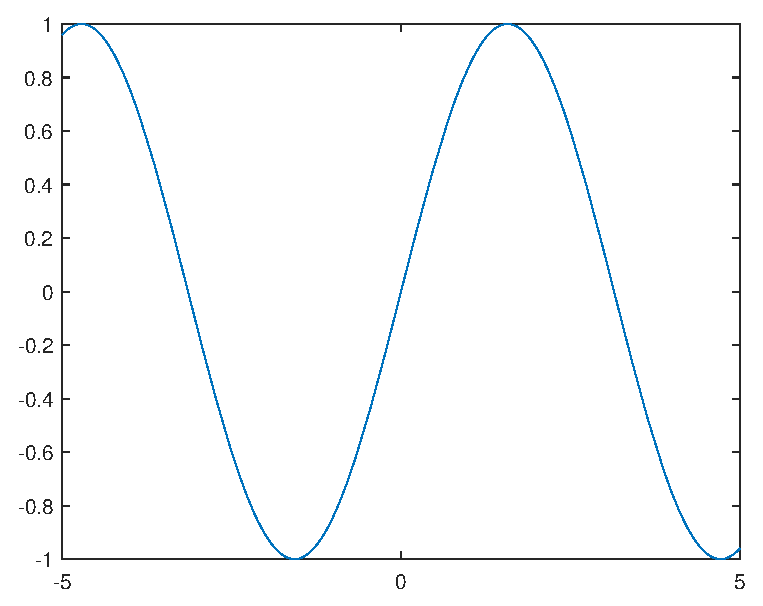
\includegraphics[width=0.6\linewidth]{image1.eps}
\end{figure}
\end{frame}

%------------------------------------------------

\begin{frame}
\frametitle{Two pictures}
\begin{figure}[htb]
\centering
\begin{minipage}{0.48\linewidth}
\centering
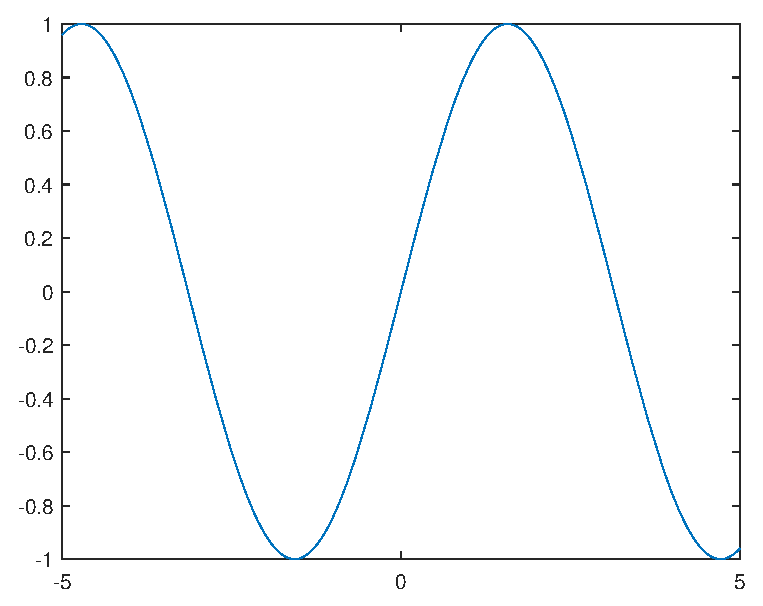
\includegraphics[width=\linewidth]{image1}
\caption{Caption of Figure 1.}
\end{minipage}\hfill
\begin{minipage}{0.48\linewidth}
\centering
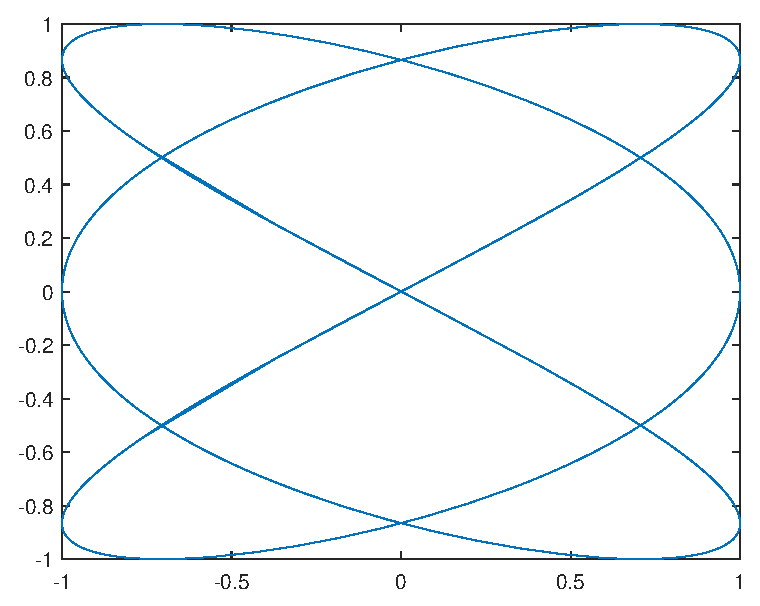
\includegraphics[width=\linewidth]{image2}
\caption{Caption of Figure 2.}
\end{minipage}
\end{figure}
\end{frame}

%------------------------------------------------
%\section{Concluding remarks}
%------------------------------------------------

\begin{frame}[fragile] % Need to use the fragile option when verbatim is used in the slide
\frametitle{Citation}
An example of the \verb|\cite| command to cite within the presentation:\\~

This statement requires citation \cite{Smith2012}.
\end{frame}

%------------------------------------------------


\begin{frame}
\frametitle{References}
\footnotesize{
\begin{thebibliography}{99} % Beamer does not support BibTeX so references must be inserted manually as below
\bibitem[Smith, 2012]{Smith2012} John Smith. Title of the publication. \emph{Journal Name}, 12(3):45--678, 2012.
\end{thebibliography}
}
\end{frame}


%------------------------------------------------
%\thispagestyle{empty}
%\setbeamertemplate{headline}{}
%\setbeamertemplate{footline}{%
%  \hfill%
%  %\usebeamercolor[fg]{page number in head/foot}%
%  \usebeamercolor[footer]{page number in head/foot}%
%  \usebeamerfont{page number in head/foot}%
%  \insertframenumber \,/\,\inserttotalframenumber
%  \kern1em\vskip2pt%
%}

%------------------------------------------------
%\setbeamertemplate{background canvas}[vertical shading][bottom=white,top=structure.fg!25]
%\setbeamertemplate{headline}{}
\begin{frame}
\rmfamily
\begin{center}
\HUGE{\textcolor[RGB]{165,3,3}{Thank~you!}}
\end{center}
\end{frame}


%------------------------------------------------

%\thispagestyle{empty}
%%\setbeamertemplate{background canvas}[vertical shading][bottom=white,top=structure.fg!25]
%\begin{frame}
%\Huge{\centerline{The End}}
%\end{frame}


\end{document}
